%%%%%%%%%%%%%%%%%%%%%%%%%%%%%%%%%%%%%%%%%
% The Legrand Orange Book
% LaTeX Template
% Version 2.0 (9/2/15)
%
% This template has been downloaded from:
% http://www.LaTeXTemplates.com
%
% Mathias Legrand (legrand.mathias@gmail.com) with modifications by:
% Vel (vel@latextemplates.com)
%
% License:
% CC BY-NC-SA 3.0 (http://creativecommons.org/licenses/by-nc-sa/3.0/)
%
% Compiling this template:
% This template uses biber for its bibliography and makeindex for its index.
% When you first open the template, compile it from the command line with the 
% commands below to make sure your LaTeX distribution is configured correctly:
%
% 1) pdflatex main
% 2) makeindex main.idx -s StyleInd.ist
% 3) biber main
% 4) pdflatex main x 2
%
% After this, when you wish to update the bibliography/index use the appropriate
% command above and make sure to compile with pdflatex several times 
% afterwards to propagate your changes to the document.
%
% This template also uses a number of packages which may need to be
% updated to the newest versions for the template to compile. It is strongly
% recommended you update your LaTeX distribution if you have any
% compilation errors.
%
% Important note:
% Chapter heading images should have a 2:1 width:height ratio,
% e.g. 920px width and 460px height.
%
%%%%%%%%%%%%%%%%%%%%%%%%%%%%%%%%%%%%%%%%%

%----------------------------------------------------------------------------------------
%	PACKAGES AND OTHER DOCUMENT CONFIGURATIONS
%----------------------------------------------------------------------------------------

\documentclass[11pt,fleqn]{book} % Default font size and left-justified equations

%----------------------------------------------------------------------------------------

%fdlkjadlkjdfsal;kjafds;lkjafsd;lkjfsad

%%%%%%%%%%%%%%%%%%%%%%%%%%%%%%%%%%%%%%%%%
% The Legrand Orange Book
% Structural Definitions File
% Version 2.0 (9/2/15)
%
% Original author:
% Mathias Legrand (legrand.mathias@gmail.com) with modifications by:
% Vel (vel@latextemplates.com)
% 
% This file has been downloaded from:
% http://www.LaTeXTemplates.com
%
% License:
% CC BY-NC-SA 3.0 (http://creativecommons.org/licenses/by-nc-sa/3.0/)
%
%%%%%%%%%%%%%%%%%%%%%%%%%%%%%%%%%%%%%%%%%

%----------------------------------------------------------------------------------------
%	VARIOUS REQUIRED PACKAGES AND CONFIGURATIONS
%----------------------------------------------------------------------------------------

\usepackage[top=3cm,bottom=3cm,left=3cm,right=3cm,headsep=10pt,a4paper]{geometry} % Page margins

\usepackage{graphicx} % Required for including pictures
\graphicspath{{Pictures/}} % Specifies the directory where pictures are stored

\usepackage{lipsum} % Inserts dummy text

\usepackage{tikz} % Required for drawing custom shapes

\usepackage[english]{babel} % English language/hyphenation

\usepackage{enumitem} % Customize lists
\setlist{nolistsep} % Reduce spacing between bullet points and numbered lists

\usepackage{booktabs} % Required for nicer horizontal rules in tables

\usepackage{xcolor} % Required for specifying colors by name
\definecolor{ocre}{RGB}{243,102,25} % Define the orange color used for highlighting throughout the book

%----------------------------------------------------------------------------------------
%	FONTS
%----------------------------------------------------------------------------------------

\usepackage{avant} % Use the Avantgarde font for headings
%\usepackage{times} % Use the Times font for headings
\usepackage{mathptmx} % Use the Adobe Times Roman as the default text font together with math symbols from the Sym­bol, Chancery and Com­puter Modern fonts

\usepackage{microtype} % Slightly tweak font spacing for aesthetics
\usepackage[utf8]{inputenc} % Required for including letters with accents
\usepackage[T1]{fontenc} % Use 8-bit encoding that has 256 glyphs

%----------------------------------------------------------------------------------------
%	BIBLIOGRAPHY AND INDEX
%----------------------------------------------------------------------------------------

\usepackage[style=alphabetic,citestyle=numeric,sorting=nyt,sortcites=true,autopunct=true,babel=hyphen,hyperref=true,abbreviate=false,backref=true,backend=biber]{biblatex}
\addbibresource{bibliography.bib} % BibTeX bibliography file
\defbibheading{bibempty}{}

\usepackage{calc} % For simpler calculation - used for spacing the index letter headings correctly
\usepackage{makeidx} % Required to make an index
\makeindex % Tells LaTeX to create the files required for indexing

%----------------------------------------------------------------------------------------
%	MAIN TABLE OF CONTENTS
%----------------------------------------------------------------------------------------

\usepackage{titletoc} % Required for manipulating the table of contents

\contentsmargin{0cm} % Removes the default margin

% Part text styling
\titlecontents{part}[0cm]
{\addvspace{20pt}\centering\large\bfseries}
{}
{}
{}

% Chapter text styling
\titlecontents{chapter}[1.25cm] % Indentation
{\addvspace{12pt}\large\sffamily\bfseries} % Spacing and font options for chapters
{\color{ocre!60}\contentslabel[\Large\thecontentslabel]{1.25cm}\color{ocre}} % Chapter number
{\color{ocre}}  
{\color{ocre!60}\normalsize\;\titlerule*[.5pc]{.}\;\thecontentspage} % Page number

% Section text styling
\titlecontents{section}[1.25cm] % Indentation
{\addvspace{3pt}\sffamily\bfseries} % Spacing and font options for sections
{\contentslabel[\thecontentslabel]{1.25cm}} % Section number
{}
{\hfill\color{black}\thecontentspage} % Page number
[]

% Subsection text styling
\titlecontents{subsection}[1.25cm] % Indentation
{\addvspace{1pt}\sffamily\small} % Spacing and font options for subsections
{\contentslabel[\thecontentslabel]{1.25cm}} % Subsection number
{}
{\ \titlerule*[.5pc]{.}\;\thecontentspage} % Page number
[]

% List of figures
\titlecontents{figure}[0em]
{\addvspace{-5pt}\sffamily}
{\thecontentslabel\hspace*{1em}}
{}
{\ \titlerule*[.5pc]{.}\;\thecontentspage}
[]

% List of tables
\titlecontents{table}[0em]
{\addvspace{-5pt}\sffamily}
{\thecontentslabel\hspace*{1em}}
{}
{\ \titlerule*[.5pc]{.}\;\thecontentspage}
[]

%----------------------------------------------------------------------------------------
%	MINI TABLE OF CONTENTS IN PART HEADS
%----------------------------------------------------------------------------------------

% Chapter text styling
\titlecontents{lchapter}[0em] % Indenting
{\addvspace{15pt}\large\sffamily\bfseries} % Spacing and font options for chapters
{\color{ocre}\contentslabel[\Large\thecontentslabel]{1.25cm}\color{ocre}} % Chapter number
{}  
{\color{ocre}\normalsize\sffamily\bfseries\;\titlerule*[.5pc]{.}\;\thecontentspage} % Page number

% Section text styling
\titlecontents{lsection}[0em] % Indenting
{\sffamily\small} % Spacing and font options for sections
{\contentslabel[\thecontentslabel]{1.25cm}} % Section number
{}
{}

% Subsection text styling
\titlecontents{lsubsection}[.5em] % Indentation
{\normalfont\footnotesize\sffamily} % Font settings
{}
{}
{}

%----------------------------------------------------------------------------------------
%	PAGE HEADERS
%----------------------------------------------------------------------------------------

\usepackage{fancyhdr} % Required for header and footer configuration

\pagestyle{fancy}
\renewcommand{\chaptermark}[1]{\markboth{\sffamily\normalsize\bfseries\chaptername\ \thechapter.\ #1}{}} % Chapter text font settings
\renewcommand{\sectionmark}[1]{\markright{\sffamily\normalsize\thesection\hspace{5pt}#1}{}} % Section text font settings
\fancyhf{} \fancyhead[LE,RO]{\sffamily\normalsize\thepage} % Font setting for the page number in the header
\fancyhead[LO]{\rightmark} % Print the nearest section name on the left side of odd pages
\fancyhead[RE]{\leftmark} % Print the current chapter name on the right side of even pages
\renewcommand{\headrulewidth}{0.5pt} % Width of the rule under the header
\addtolength{\headheight}{2.5pt} % Increase the spacing around the header slightly
\renewcommand{\footrulewidth}{0pt} % Removes the rule in the footer
\fancypagestyle{plain}{\fancyhead{}\renewcommand{\headrulewidth}{0pt}} % Style for when a plain pagestyle is specified

% Removes the header from odd empty pages at the end of chapters
\makeatletter
\renewcommand{\cleardoublepage}{
\clearpage\ifodd\c@page\else
\hbox{}
\vspace*{\fill}
\thispagestyle{empty}
\newpage
\fi}

%----------------------------------------------------------------------------------------
%	THEOREM STYLES
%----------------------------------------------------------------------------------------

\usepackage{amsmath,amsfonts,amssymb,amsthm} % For math equations, theorems, symbols, etc

\newcommand{\intoo}[2]{\mathopen{]}#1\,;#2\mathclose{[}}
\newcommand{\ud}{\mathop{\mathrm{{}d}}\mathopen{}}
\newcommand{\intff}[2]{\mathopen{[}#1\,;#2\mathclose{]}}
\newtheorem{notation}{Notation}[chapter]

% Boxed/framed environments
\newtheoremstyle{ocrenumbox}% % Theorem style name
{0pt}% Space above
{0pt}% Space below
{\normalfont}% % Body font
{}% Indent amount
{\small\bf\sffamily\color{ocre}}% % Theorem head font
{\;}% Punctuation after theorem head
{0.25em}% Space after theorem head
{\small\sffamily\color{ocre}\thmname{#1}\nobreakspace\thmnumber{\@ifnotempty{#1}{}\@upn{#2}}% Theorem text (e.g. Theorem 2.1)
\thmnote{\nobreakspace\the\thm@notefont\sffamily\bfseries\color{black}---\nobreakspace#3.}} % Optional theorem note
\renewcommand{\qedsymbol}{$\blacksquare$}% Optional qed square

\newtheoremstyle{blacknumex}% Theorem style name
{5pt}% Space above
{5pt}% Space below
{\normalfont}% Body font
{} % Indent amount
{\small\bf\sffamily}% Theorem head font
{\;}% Punctuation after theorem head
{0.25em}% Space after theorem head
{\small\sffamily{\tiny\ensuremath{\blacksquare}}\nobreakspace\thmname{#1}\nobreakspace\thmnumber{\@ifnotempty{#1}{}\@upn{#2}}% Theorem text (e.g. Theorem 2.1)
\thmnote{\nobreakspace\the\thm@notefont\sffamily\bfseries---\nobreakspace#3.}}% Optional theorem note

\newtheoremstyle{blacknumbox} % Theorem style name
{0pt}% Space above
{0pt}% Space below
{\normalfont}% Body font
{}% Indent amount
{\small\bf\sffamily}% Theorem head font
{\;}% Punctuation after theorem head
{0.25em}% Space after theorem head
{\small\sffamily\thmname{#1}\nobreakspace\thmnumber{\@ifnotempty{#1}{}\@upn{#2}}% Theorem text (e.g. Theorem 2.1)
\thmnote{\nobreakspace\the\thm@notefont\sffamily\bfseries---\nobreakspace#3.}}% Optional theorem note

% Non-boxed/non-framed environments
\newtheoremstyle{ocrenum}% % Theorem style name
{5pt}% Space above
{5pt}% Space below
{\normalfont}% % Body font
{}% Indent amount
{\small\bf\sffamily\color{ocre}}% % Theorem head font
{\;}% Punctuation after theorem head
{0.25em}% Space after theorem head
{\small\sffamily\color{ocre}\thmname{#1}\nobreakspace\thmnumber{\@ifnotempty{#1}{}\@upn{#2}}% Theorem text (e.g. Theorem 2.1)
\thmnote{\nobreakspace\the\thm@notefont\sffamily\bfseries\color{black}---\nobreakspace#3.}} % Optional theorem note
\renewcommand{\qedsymbol}{$\blacksquare$}% Optional qed square
\makeatother

% Defines the theorem text style for each type of theorem to one of the three styles above
\newcounter{dummy} 
\numberwithin{dummy}{section}
\theoremstyle{ocrenumbox}
\newtheorem{theoremeT}[dummy]{Theorem}
\newtheorem{problem}{Problem}[chapter]
\newtheorem{exerciseT}{Exercise}[chapter]
\theoremstyle{blacknumex}
\newtheorem{exampleT}{Example}[chapter]
\theoremstyle{blacknumbox}
\newtheorem{vocabulary}{Vocabulary}[chapter]
\newtheorem{definitionT}{Definition}[section]
\newtheorem{corollaryT}[dummy]{Corollary}
\theoremstyle{ocrenum}
\newtheorem{proposition}[dummy]{Proposition}

%----------------------------------------------------------------------------------------
%	DEFINITION OF COLORED BOXES
%----------------------------------------------------------------------------------------

\RequirePackage[framemethod=default]{mdframed} % Required for creating the theorem, definition, exercise and corollary boxes

% Theorem box
\newmdenv[skipabove=7pt,
skipbelow=7pt,
backgroundcolor=black!5,
linecolor=ocre,
innerleftmargin=5pt,
innerrightmargin=5pt,
innertopmargin=5pt,
leftmargin=0cm,
rightmargin=0cm,
innerbottommargin=5pt]{tBox}

% Exercise box	  
\newmdenv[skipabove=7pt,
skipbelow=7pt,
rightline=false,
leftline=true,
topline=false,
bottomline=false,
backgroundcolor=ocre!10,
linecolor=ocre,
innerleftmargin=5pt,
innerrightmargin=5pt,
innertopmargin=5pt,
innerbottommargin=5pt,
leftmargin=0cm,
rightmargin=0cm,
linewidth=4pt]{eBox}	

% Definition box
\newmdenv[skipabove=7pt,
skipbelow=7pt,
rightline=false,
leftline=true,
topline=false,
bottomline=false,
linecolor=ocre,
innerleftmargin=5pt,
innerrightmargin=5pt,
innertopmargin=0pt,
leftmargin=0cm,
rightmargin=0cm,
linewidth=4pt,
innerbottommargin=0pt]{dBox}	

% Corollary box
\newmdenv[skipabove=7pt,
skipbelow=7pt,
rightline=false,
leftline=true,
topline=false,
bottomline=false,
linecolor=gray,
backgroundcolor=black!5,
innerleftmargin=5pt,
innerrightmargin=5pt,
innertopmargin=5pt,
leftmargin=0cm,
rightmargin=0cm,
linewidth=4pt,
innerbottommargin=5pt]{cBox}

% Creates an environment for each type of theorem and assigns it a theorem text style from the "Theorem Styles" section above and a colored box from above
\newenvironment{theorem}{\begin{tBox}\begin{theoremeT}}{\end{theoremeT}\end{tBox}}
\newenvironment{exercise}{\begin{eBox}\begin{exerciseT}}{\hfill{\color{ocre}\tiny\ensuremath{\blacksquare}}\end{exerciseT}\end{eBox}}				  
\newenvironment{definition}{\begin{dBox}\begin{definitionT}}{\end{definitionT}\end{dBox}}	
\newenvironment{example}{\begin{exampleT}}{\hfill{\tiny\ensuremath{\blacksquare}}\end{exampleT}}		
\newenvironment{corollary}{\begin{cBox}\begin{corollaryT}}{\end{corollaryT}\end{cBox}}	

%----------------------------------------------------------------------------------------
%	REMARK ENVIRONMENT
%----------------------------------------------------------------------------------------

\newenvironment{remark}{\par\vspace{10pt}\small % Vertical white space above the remark and smaller font size
\begin{list}{}{
\leftmargin=35pt % Indentation on the left
\rightmargin=25pt}\item\ignorespaces % Indentation on the right
\makebox[-2.5pt]{\begin{tikzpicture}[overlay]
\node[draw=ocre!60,line width=1pt,circle,fill=ocre!25,font=\sffamily\bfseries,inner sep=2pt,outer sep=0pt] at (-15pt,0pt){\textcolor{ocre}{R}};\end{tikzpicture}} % Orange R in a circle
\advance\baselineskip -1pt}{\end{list}\vskip5pt} % Tighter line spacing and white space after remark

%----------------------------------------------------------------------------------------
%	SECTION NUMBERING IN THE MARGIN
%----------------------------------------------------------------------------------------

\makeatletter
\renewcommand{\@seccntformat}[1]{\llap{\textcolor{ocre}{\csname the#1\endcsname}\hspace{1em}}}                    
\renewcommand{\section}{\@startsection{section}{1}{\z@}
{-4ex \@plus -1ex \@minus -.4ex}
{1ex \@plus.2ex }
{\normalfont\large\sffamily\bfseries}}
\renewcommand{\subsection}{\@startsection {subsection}{2}{\z@}
{-3ex \@plus -0.1ex \@minus -.4ex}
{0.5ex \@plus.2ex }
{\normalfont\sffamily\bfseries}}
\renewcommand{\subsubsection}{\@startsection {subsubsection}{3}{\z@}
{-2ex \@plus -0.1ex \@minus -.2ex}
{.2ex \@plus.2ex }
{\normalfont\small\sffamily\bfseries}}                        
\renewcommand\paragraph{\@startsection{paragraph}{4}{\z@}
{-2ex \@plus-.2ex \@minus .2ex}
{.1ex}
{\normalfont\small\sffamily\bfseries}}

%----------------------------------------------------------------------------------------
%	PART HEADINGS
%----------------------------------------------------------------------------------------

% numbered part in the table of contents
\newcommand{\@mypartnumtocformat}[2]{%
\setlength\fboxsep{0pt}%
\noindent\colorbox{ocre!20}{\strut\parbox[c][.7cm]{\ecart}{\color{ocre!70}\Large\sffamily\bfseries\centering#1}}\hskip\esp\colorbox{ocre!40}{\strut\parbox[c][.7cm]{\linewidth-\ecart-\esp}{\Large\sffamily\centering#2}}}%
%%%%%%%%%%%%%%%%%%%%%%%%%%%%%%%%%%
% unnumbered part in the table of contents
\newcommand{\@myparttocformat}[1]{%
\setlength\fboxsep{0pt}%
\noindent\colorbox{ocre!40}{\strut\parbox[c][.7cm]{\linewidth}{\Large\sffamily\centering#1}}}%
%%%%%%%%%%%%%%%%%%%%%%%%%%%%%%%%%%
\newlength\esp
\setlength\esp{4pt}
\newlength\ecart
\setlength\ecart{1.2cm-\esp}
\newcommand{\thepartimage}{}%
\newcommand{\partimage}[1]{\renewcommand{\thepartimage}{#1}}%
\def\@part[#1]#2{%
\ifnum \c@secnumdepth >-2\relax%
\refstepcounter{part}%
\addcontentsline{toc}{part}{\texorpdfstring{\protect\@mypartnumtocformat{\thepart}{#1}}{\partname~\thepart\ ---\ #1}}
\else%
\addcontentsline{toc}{part}{\texorpdfstring{\protect\@myparttocformat{#1}}{#1}}%
\fi%
\startcontents%
\markboth{}{}%
{\thispagestyle{empty}%
\begin{tikzpicture}[remember picture,overlay]%
\node at (current page.north west){\begin{tikzpicture}[remember picture,overlay]%	
\fill[ocre!20](0cm,0cm) rectangle (\paperwidth,-\paperheight);
\node[anchor=north] at (4cm,-3.25cm){\color{ocre!40}\fontsize{220}{100}\sffamily\bfseries\@Roman\c@part}; 
\node[anchor=south east] at (\paperwidth-1cm,-\paperheight+1cm){\parbox[t][][t]{8.5cm}{
\printcontents{l}{0}{\setcounter{tocdepth}{1}}%
}};
\node[anchor=north east] at (\paperwidth-1.5cm,-3.25cm){\parbox[t][][t]{15cm}{\strut\raggedleft\color{white}\fontsize{30}{30}\sffamily\bfseries#2}};
\end{tikzpicture}};
\end{tikzpicture}}%
\@endpart}
\def\@spart#1{%
\startcontents%
\phantomsection
{\thispagestyle{empty}%
\begin{tikzpicture}[remember picture,overlay]%
\node at (current page.north west){\begin{tikzpicture}[remember picture,overlay]%	
\fill[ocre!20](0cm,0cm) rectangle (\paperwidth,-\paperheight);
\node[anchor=north east] at (\paperwidth-1.5cm,-3.25cm){\parbox[t][][t]{15cm}{\strut\raggedleft\color{white}\fontsize{30}{30}\sffamily\bfseries#1}};
\end{tikzpicture}};
\end{tikzpicture}}
\addcontentsline{toc}{part}{\texorpdfstring{%
\setlength\fboxsep{0pt}%
\noindent\protect\colorbox{ocre!40}{\strut\protect\parbox[c][.7cm]{\linewidth}{\Large\sffamily\protect\centering #1\quad\mbox{}}}}{#1}}%
\@endpart}
\def\@endpart{\vfil\newpage
\if@twoside
\if@openright
\null
\thispagestyle{empty}%
\newpage
\fi
\fi
\if@tempswa
\twocolumn
\fi}

%----------------------------------------------------------------------------------------
%	CHAPTER HEADINGS
%----------------------------------------------------------------------------------------

\newcommand{\thechapterimage}{}%
\newcommand{\chapterimage}[1]{\renewcommand{\thechapterimage}{#1}}%
\def\@makechapterhead#1{%
{\parindent \z@ \raggedright \normalfont
\ifnum \c@secnumdepth >\m@ne
\if@mainmatter
\begin{tikzpicture}[remember picture,overlay]
\node at (current page.north west)
{\begin{tikzpicture}[remember picture,overlay]
\node[anchor=north west,inner sep=0pt] at (0,0) {\includegraphics[width=\paperwidth]{\thechapterimage}};
\draw[anchor=west] (\Gm@lmargin,-9cm) node [line width=2pt,rounded corners=15pt,draw=ocre,fill=white,fill opacity=0.5,inner sep=15pt]{\strut\makebox[22cm]{}};
\draw[anchor=west] (\Gm@lmargin+.3cm,-9cm) node {\huge\sffamily\bfseries\color{black}\thechapter. #1\strut};
\end{tikzpicture}};
\end{tikzpicture}
\else
\begin{tikzpicture}[remember picture,overlay]
\node at (current page.north west)
{\begin{tikzpicture}[remember picture,overlay]
\node[anchor=north west,inner sep=0pt] at (0,0) {\includegraphics[width=\paperwidth]{\thechapterimage}};
\draw[anchor=west] (\Gm@lmargin,-9cm) node [line width=2pt,rounded corners=15pt,draw=ocre,fill=white,fill opacity=0.5,inner sep=15pt]{\strut\makebox[22cm]{}};
\draw[anchor=west] (\Gm@lmargin+.3cm,-9cm) node {\huge\sffamily\bfseries\color{black}#1\strut};
\end{tikzpicture}};
\end{tikzpicture}
\fi\fi\par\vspace*{270\p@}}}

%-------------------------------------------

\def\@makeschapterhead#1{%
\begin{tikzpicture}[remember picture,overlay]
\node at (current page.north west)
{\begin{tikzpicture}[remember picture,overlay]
\node[anchor=north west,inner sep=0pt] at (0,0) {\includegraphics[width=\paperwidth]{\thechapterimage}};
\draw[anchor=west] (\Gm@lmargin,-9cm) node [line width=2pt,rounded corners=15pt,draw=ocre,fill=white,fill opacity=0.5,inner sep=15pt]{\strut\makebox[22cm]{}};
\draw[anchor=west] (\Gm@lmargin+.3cm,-9cm) node {\huge\sffamily\bfseries\color{black}#1\strut};
\end{tikzpicture}};
\end{tikzpicture}
\par\vspace*{270\p@}}
\makeatother

%----------------------------------------------------------------------------------------
%	HYPERLINKS IN THE DOCUMENTS
%----------------------------------------------------------------------------------------

\usepackage{hyperref}
\hypersetup{hidelinks,backref=true,pagebackref=true,hyperindex=true,colorlinks=false,breaklinks=true,urlcolor= ocre,bookmarks=true,bookmarksopen=false,pdftitle={Title},pdfauthor={Author}}
\usepackage{bookmark}
\bookmarksetup{
open,
numbered,
addtohook={%
\ifnum\bookmarkget{level}=0 % chapter
\bookmarksetup{bold}%
\fi
\ifnum\bookmarkget{level}=-1 % part
\bookmarksetup{color=ocre,bold}%
\fi
}
}
 % Insert the commands.tex file which contains the majority of the structure behind the template

\begin{document}

%----------------------------------------------------------------------------------------
%	TITLE PAGE
%----------------------------------------------------------------------------------------

\begingroup
\thispagestyle{empty}
\begin{tikzpicture}[remember picture,overlay]
\coordinate [below=12cm] (midpoint) at (current page.north);
\node at (current page.north west)
{\begin{tikzpicture}[remember picture,overlay]
\node[anchor=north west,inner sep=0pt] at (0,0) {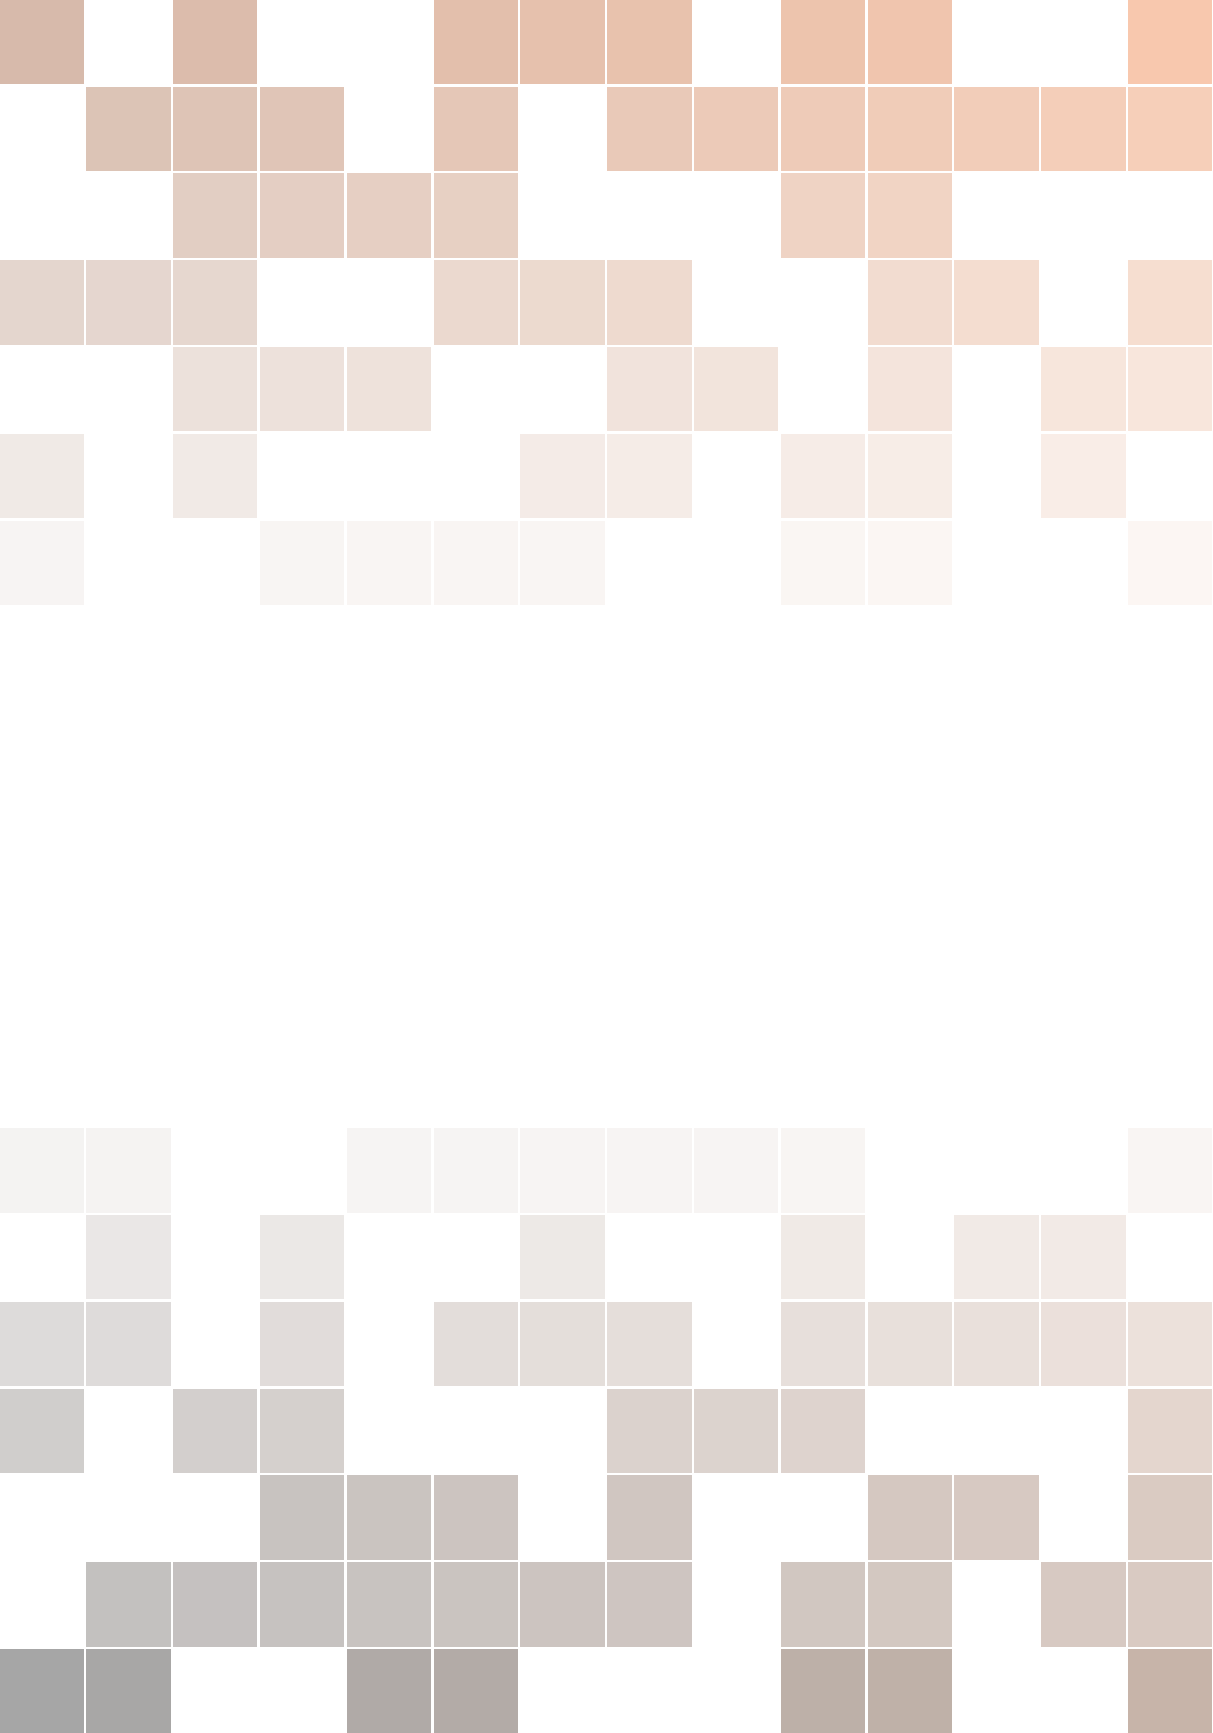
\includegraphics[width=\paperwidth]{background}}; % Background image
\draw[anchor=north] (midpoint) node [fill=ocre!30!white,fill opacity=0.6,text opacity=1,inner sep=1cm]{\Huge\centering\bfseries\sffamily\parbox[c][][t]{\paperwidth}{\centering Theory of Statistics I\\[15pt] % Book title
{\Large Take Two}\\[20pt] % Subtitle
{\huge Meridith L Bartley}}}; % Author name
\end{tikzpicture}};
\end{tikzpicture}
\vfill
\endgroup

%----------------------------------------------------------------------------------------
%	COPYRIGHT PAGE
%----------------------------------------------------------------------------------------

\newpage
~\vfill
\thispagestyle{empty}

\noindent Copyright \copyright\ 2013 Meridith L Bartley\\ % Copyright notice

\noindent \textsc{Published by Publisher}\\ % Publisher

\noindent \textsc{book-website.com}\\ % URL

\noindent Licensed under the Creative Commons Attribution-NonCommercial 3.0 Unported License (the ``License''). You may not use this file except in compliance with the License. You may obtain a copy of the License at \url{http://creativecommons.org/licenses/by-nc/3.0}. Unless required by applicable law or agreed to in writing, software distributed under the License is distributed on an \textsc{``as is'' basis, without warranties or conditions of any kind}, either express or implied. See the License for the specific language governing permissions and limitations under the License.\\ % License information

\noindent \textit{First printing, August 2015} % Printing/edition date

%----------------------------------------------------------------------------------------
%	TABLE OF CONTENTS
%----------------------------------------------------------------------------------------

\chapterimage{chapter_head_1.pdf} % Table of contents heading image

\pagestyle{empty} % No headers

\tableofcontents % Print the table of contents itself

\cleardoublepage % Forces the first chapter to start on an odd page so it's on the right

\pagestyle{fancy} % Print headers again

%----------------------------------------------------------------------------------------
%	PART
%----------------------------------------------------------------------------------------

\part{Part One}

%----------------------------------------------------------------------------------------
%	CHAPTER 1
%----------------------------------------------------------------------------------------

\chapterimage{chapter_head_2.pdf} % Chapter heading image

\chapter{Real Analysis Review}

\section{The Real Number System}\index{The Real Number System}
\subsection{Rationals}\index{Rationals}


Start with integers as given. 

\begin{definition}[Rational Numbers]
Rationals are numbers of the form $\frac{m}{n}$, for m,n integers, $n \neq 0$ such that:
\begin{align*}
& \text{PR 1: The sum, difference, product, and ratio (division by 0 excluded) of any two rationals is a rational.}\\
& \text{PR 2: } p+q = q+p, pq=qp \text{ (Commutative Property)}\\
& \text{PR 3: } (p+q)+r = p+(q+r), (pq)r = p(qr), \text{ (Associative Property)} \\
& \text{PR 4: } (p+q)r = pr + qr \text{ (Distributive Property)} \\
& \text{PR 5: } \forall \text{ two rationals p and q we have either p=q, p<q, or q<p (Ordering Property)} \\
& \text{PR 6: If $p<q$ and $q<r$, then $p<r$ (Transitivity of <)}\\
& \text{PR 7: If $p>0$ and $q>0$, then $p+q>0$ and $pq >0$} \\
& \text{PR 8: If $p<q$, then $p+r<q+r$  $\forall$ r} \\
\end{align*}
\end{definition}

The rational number system is inadequate. 

\begin{example}
	There is no rational number p that satisfies $p^2 = 2$
\end{example}

	\begin{proof}
		Suppose such a p existed, and so $p=\frac{m}{n}$. Note that m,n can be chosen so not both are even. Then we have,
		$$m^2 = 2n^2 $$
		Thus, $m^2$ is even, and hence m is even. (The square of an odd number is odd). Hence, $m^2$ is divided by 4. So, $2n^2$ is divisible by 4, or $n^2$ is even which implies that n is even - $\textbf{contradiction}$.
	\end{proof}

This example can be used to show that we can have a set of rational numbers bounded from above but has no supremum. 

\begin{example}
	Let A be the set of $<0$ rationals p, such that $p^2 <2$. Let B be the set of $>0$ rationals p, such that $p^2 >2$. Then A contains no largest number and B contains no smallest number.
\end{example}

\begin{proof}
	If $p \in A$, choose a rational h such that, $0<h<1$ and $h<\frac{2-p^2}{2p+1}$ and set $q=p+h$. Then q is rational and 
	\begin{align*}
		q^2 &= p^2 + (2p+h)h\\
		&< p^2 + (2p+1)h\\
		&< p^2 + (2-p^2)\\
		&= 2
	\end{align*}
	If $p \in B$, set
	
	\begin{align*}
			 q= p- \frac{p^2 - 2}{2p} = \frac{p}{2} + \frac{1}{p}
	\end{align*}
	and
	\begin{align*}
		q^2 &= p^2 - (p^2 - 2) + (\frac{p^2 - 2}{2p})^2\\
		&> p^2 - (p^2 -2)\\
		&= 2
	\end{align*}
\end{proof}

\begin{remark}
	An axiomatic treatment of the real number system uses PR1 - PR8 as axioms together with the "completeness axiom". The non-axiomatics treatment is due to Dedekind.
\end{remark}


\subsection{Sets and Subsets}\index{Sets and Subsets}

If A is any set, $\mathbf{x \in A}$ means that x is a member of A, and $\mathbf{x \notin A}$ means x is not a member of A. A set B is a \textbf{subset} of A if for every $x \in B$ we have $x \in A$, and we write $A \subseteq B$. B is a \textbf{proper subset} of A, $B \subset A$, if there $\exists$ $x \in A$ with $x \notin B$. The \textbf{empty set} is denoted by $\emptyset$, and $\emptyset \in A$, $\forall$ other set A.

\begin{align*}
	A \cup B &= B \cup A \text{ - union with commutative property}\\
	\\
	A \cap B &= B \cap A \text{ - intersection with commutative property}\\
	\\
	(A \cup B)\cup C &= A\cup(B \cup C)\\
	(A \cap B)\cap C &= A\cap(B \cap C) \text{ - associative property}\\
	\\
	 (A \cup B)\cap C &= (A\cap C)\cup(B \cap C) \text{ - distributive property}\\
	 (\cup A_i)^c &= \cap A_i^c\\
	 (\cap A_i)^c &= \cup A_i^c\\
\end{align*}

\begin{definition}[Dedekind Cuts]
	A set $\alpha$ of rational numbers is said to be a \textbf{cut} if
	\begin{enumerate}[label = \alph*)]
		\item $\alpha$ is a proper, but non-empty, subset of the rational numbers.
		\item If $p \in \alpha$ (p is rational), and $q<p$ (q is rational) then $q \in \alpha$
		\item It contains no largest rational.
	\end{enumerate}
	A cut of the form $\alpha$ = $\{$p: p is rational and $p<r\}$ where r is rational are called \textbf{rational cuts} and are denoted by $r^*$.
\end{definition}

The development of the real number system proceeds as follows:\\
First, the set of cuts is equipped with an order relation, and the operation of addition and multiplication an it will show that the resulting arethmatic satisfies PR 1 - PR 8.  

If $\alpha$, $\beta$ are cuts then, 
\begin{align*}
	\alpha &< \beta \text{ if $\alpha \subset \beta$ and} \\
	\alpha &\le \beta \text{ if $\alpha \subseteq \beta$}\\
	\alpha + \beta &= \{r: r= p + q \text{ for some } p \in \alpha, q \in \beta\}\\
	(\alpha + 0^* &= \alpha)
\end{align*}

If $\alpha + \beta = 0^*$, write $\beta = -\alpha$. (It can be shown that $\forall \alpha$ there is one and only one $\beta$ such that $\alpha + \beta = 0^*$.) 
$$|\alpha| = \begin{cases}
  \alpha, & \text{if } \alpha \ge 0^*, \\
  -\alpha, & \text{if } \alpha < 0^* .
\end{cases} $$

For $\alpha \ge 0^*$ and $\beta \ge 0^*$, 
$$\alpha\beta = \{\text{p:p rational such that either $p<0$ or $p=pq$, for $q \in \alpha$, $r \in \beta$ with $q \ge 0$ and $r \ge 0$.}\}$$ 

For general $\alpha$, $\beta$,
$$\alpha\beta = \begin{cases}
  -(|\alpha||\beta|), & \text{if } \alpha < 0^*, \text{and } \beta \ge 0^*\\
  	& \text{or if } \alpha \ge 0^* \text{and } \beta < 0^*\\
  |\alpha||\beta|, & \text{if } \alpha < 0^*, \text{and } \beta < 0^*\\
\end{cases} $$

If $\alpha \neq 0^*$, then $\forall \beta$ there is one and only one $\gamma$ such that $\alpha\gamma = \beta$, and this $\gamma$ is denoted by $\frac{\beta}{\alpha}$. (In technical terms, we made the set of cuts an \textbf{ordered field}.)

Second, it is shown that replacing the set of rational numbers by the corresponding cuts preserves sums, products and order, ie,

\begin{enumerate}
	\item $p^* + q^* =(p + q)^*$ 
	\item $p^*q^* = (pq)^*$
	\item $p^* < q^*$ iff $p<q$
\end{enumerate}
In technical terms, the ordered field of rational numbers is \textbf{isomorphic} to that of rational events.

\begin{theorem}[Dedekind]
	Let A, B be $\subset \mathbb{R}$ such that,
	\begin{enumerate}[label = (\alph*)]
		\item $A \cap B = \emptyset$
		\item $A \cup B = \mathbb{R}$
		\item neither $A$ nor $B$ is empty
		\item if $\alpha \in A$, $\beta \in B$, then $\alpha < \beta$
	\end{enumerate}
	Then there $\exists$ $\gamma \in \mathbb{R}$ such that $\alpha \le \gamma$, $\forall \alpha \in A$ and $\gamma \le \beta$, $\forall \beta \in B$. 
\end{theorem}

\begin{proof}
	First, suppose there are 2 $\gamma$, say $\gamma_1 < \gamma_2$. Take $\gamma_3$ such that $\gamma_1 < \gamma_3 < \gamma_2$.
	$$\gamma_3 < \gamma_2 \text{ implies that } \gamma_3 \in A$$
	$$\gamma_1 < \gamma_3 \text{ implies that } \gamma_3 \in B$$
However, these implications contradict the disjointness (part (a)). 
Define $\gamma - \{\text{p: p rational such that p }\in \alpha \text{ for some }\alpha \in A\}$. The proof proceeds by showing that $\gamma$ is a cut, and hense a real number that satisfies $\alpha \le \gamma$ for $\alpha \in A$ and $\gamma \le \beta$ $\forall$ $\beta \in B$.
\end{proof}

\begin{corollary}
	If A, B are as in the theorem, then either A contains a largest number or B contains a smallest number. 
\end{corollary}

\begin{corollary}	
	Let $E \neq \emptyset$ be a subset of $\mathbb{R}$. Then, if E is bounded above a supremum (least upper bound) exists.
\end{corollary}	

\begin{proof}
	Define \\
	$A = \{\alpha: \alpha < x \text{ for some }x \in E\}$\\
	$B = A^c$\\
	Clearly, all members of B are upper bounds of E. It is sufficient to prove that B contains a smallest nubmer, or, by Corollary 1, that A does not contain a largest number (and thus prove by contradiction). Indeed if $\alpha \in A$ $\exists$ an $x \in E$ such that $\alpha < x$. But, by Property 1 (???) there $\exists$ an $\alpha^\prime$ such that $\alpha < \alpha^\prime < x$ where $\alpha^\prime \in A $ (i.e. we can always find a larger $\alpha$ so, since there is no largest $\alpha$, there MUST be a smallest $\beta$).  
\end{proof}

\begin{theorem}
	Any real number admits a decimal expansion.
\end{theorem}

\begin{proof}
	Let $x > 0$, $x \in \mathbb{R}$. Let $n_0 = [x]$ (n largest integer < x). Let $n_1$ be the largest integer such that $n_0 + \frac{n_1}{10} < x$. Having defined $n_0 \dots n_{k-1}$, define $n_k$ as the largest integer such that $n_0 + \frac{n_1}{10} + \frac{n_2}{10^2} + \dots + \frac{n_k}{1-^k} \le x$. Let E bet he set of resluting numbers for $k=1,2,\dots$. Then $x$ is the supremum of E and $n_0, n_1, \dots$ is its \textbf{decimal expansion}. Conversely, and set of integers $n_0, n_1, \dots$ defines a set of numbers, E, bounded above by $n_0 + 1$.	
\end{proof}

\begin{definition}[Extended Real Number System]
	$$\bar{\mathbb{R}} = \mathbb{R} \cup \{-\infty, \infty\}$$
\end{definition}

\subsection{Euclidean Space}\index{Euclidean Space}

\begin{definition}[Vector Space]
	For any $k \in \mathbb{Z}^+$. Let $\mathbb{R}^K$ be the set of ordered k-tuples. 
	\begin{align*}
	\underline{x} &= (x_1, \dots, x_k) \text{ with }x_i \in \mathbb{R}\\
	\underline{y} &= (y_1, \dots, y_k) \alpha \in \mathbb{R}\\
	\underline{x} + \underline{y} &= (x_1 + y_1, \dots, x_k + y_k)\\
	\alpha\underline{x} &	= (\alpha x_1, \dots, \alpha x_k)\\
	\end{align*}
	Which makes $\mathbb{R}^k$ a \textbf{vector space} over the \textbf{real field}.
\end{definition}

\begin{definition}[Inner/Scalar/Dot Product]
$$ \underline{x} \cdot \underline{y} = \sum\limits_{i=1}^k x_i y_i$$	
\end{definition}

\begin{definition}[Norm/Length]
	$$|\underline{x}| = (\underline{x}\underline{x})^{\frac{1}{2}} = \sqrt{\sum\limits_{i=1}^k x_i^2} $$
\end{definition}

\begin{definition}[Euclidean K-space]
	The vector space $\mathbb{R}^k$ with the inner product and norm is called \textbf{Euclidean k-space}.
\end{definition}

\begin{theorem}
	For $\underline{x}, \underline{y} \in \mathbb{R}^k, \alpha \in \mathbb{R}$
	\begin{enumerate}[label = \alph*)]
		\item $|\underline{x}| \ge 0, |\underline{x}| = 0 \text{ iff } \underline{x} = \underline{0}$\\
		$|\alpha \underline{x}| = |\underline{\alpha}||\underline{x}|$ 
		\item \textbf{Cauchy-Schwarz Inequality} $|\underline{x}\cdot\underline{y}| \le |\underline{x}||\underline{y}|$
		\item \textbf{Triangle Inequality} $|\underline{x}+\underline{y}| \le |\underline{x}| + |\underline{y}|$
	\end{enumerate}
\end{theorem}

\section{Elements of Set Theory}\index{Elements of Set Theory}

\begin{definition}
	Let A, B be sets and suppose that to each $x \in A$ there corresponds an elements of B denoted by $f(x)$. Then $f$ is a \textbf{function} (or in more general space, mapping) from A (in)to B. 

	A is called the \textbf{domain} of $f$. $f(x)$ is the \textbf{value} of $f$ at $x$, $R(f) = \{f(x): x \in A\}$ is the \textbf{range} of $f$.
\end{definition}

\begin{definition}[Image]
	If $f$ is a function from A to B ($A \rightarrow B$) and $E \subseteq A$ we write $f(E) = \{f(x): x \in E\}$ and call it the \textbf{image} of E under $f$.
	If $f(A) = B$, then we say $f$ maps A \textbf{onto} B.
\end{definition}

\begin{definition}[Inverse Image]
	Let $f: A \rightarrow B$ and $E \subseteq B$. We write $f^{-1}(E) = \{x ]in A : f(x) \in E\}$ and call it the \textbf{inverse image} of E \textbf{under} $f$.
	NB: If $E =\{y\}, y \in B$ we also write $f^{-1}(y)$ (versus $f^{-1}(\{y\})$). If $\forall y \in B$ $f^{-1}(y)$ consists of at most one element, then $f$ is one to one mapping of A \textbf{into} B.
\end{definition}

\begin{theorem}  
	\begin{enumerate}[label = \alph*)]
		\item $f^{-1}(A\cup B) = f^{-1}(A)\cup f^{-1}(B)$
		\item $f(A\cup B) = f(A) \cup f(B)$
		\item $f^{-1}(A\cap B) = f^{-1}(A) \cap f^{-1}(B)$
	\end{enumerate}
	Actually, these may be extended to arbitrary unions and intersections.
	\begin{align*}	
		f^{-1}(\bigcup\limits_\alpha A_\alpha) &= \bigcup_\alpha f^{-1}(A_\alpha)\\
		f^{-1} (\bigcap_\alpha A_\alpha) &= \bigcap_\alpha f^{-1}(A_\alpha)\\
		f(\bigcup_\alpha A_\alpha) &= \bigcup_\alpha f(A_\alpha)
	\end{align*}	
	Note: $f(A\cap B)$ is not necessarily equal to $f(A) \cap f(B)$ (see notes for example and sketch)
\end{theorem}

\begin{definition}[Cardinal Number]
	If $\exists$ a one-to-one mapping of A onto B, we say that A and B have the same \textbf{cardinal number}, or that they are \textbf{equivalent} $A\sim B$.  
	\begin{enumerate}[label = \alph*)]
		\item $A \sim A$ (reflective)
		\item If $A \sim B$, then $B \sim A$ (symmetric)
		\item If $A \sim B$ and $B \sim C$, then $A \sim C$. (transitive)
	\end{enumerate}
\end{definition}

\begin{definition}[(In)finite/(Un)Countable]
	Let $\mathbb{Z}^+ = \{1, 2, \dots \}$ and $\mathbb{Z}_n^+ = \{1, 2, \dots, n\}$ and let A be a set.
	\begin{enumerate}[label = \alph*)]
		\item We say A is \textbf{finite} if $A \sim \mathbb{Z}^+_n$ for some n or if $A = \emptyset$
		\item A is \textbf{infinite} if it is not finite
		\item A is \textbf{countable} if $A \sim \mathbb{Z}^+$
		\item A is \textbf{uncountable} if A is not finite and countable.
	\end{enumerate}
	Note: If A and B are finite, then $A \sim B$ if and only if they have the same number of elements. This is not true if they are infinite. 
\end{definition}

\begin{example}
	\textbf{Equivalent Infinite Sets}
	\begin{enumerate}
		\item The set $\mathbb{Z}^+$ of all integers is countable. Then take
			 $$ f(x) = \begin{cases}
	  		\frac{n}{2}, & \text{if n is even} \\
	  		-(\frac{n-1}{2}), & \text{if n is odd} 
			\end{cases} $$
			\end{enumerate}

			\begin{table}[h]
			\centering
			\begin{tabular}{l l l}
			1 & $\rightarrow$ & 0 \\
			2 & $\rightarrow$ & 1 \\
			3 & $\rightarrow$ & -1 \\
			4 & $\rightarrow$ & 2 \\
			5 & $\rightarrow$ & -2 \\
			6 & $\rightarrow$ & 3 \\
			7 & $\rightarrow$ & -3 \\
			\end{tabular}
			\caption{Corresponding Integers}
			\end{table}
		\item The set of positive, even integers is countable. Take
	$$f(x)=2n $$	
\end{example}

\begin{theorem}
	The countable union of countable sets is countable.
\end{theorem}

\begin{proof}
	Let $A_1, A_2, \dots$ be countable and assume that they are disjoint (for if not, you can consider the sequences of countable sets that are disjoint - $A_1, A_2-A_1, \dots$), which are countable and have the same union. 
	Let $A_k = \{a_{k1}, a_{k2}, \dots\}$ and consider the arrangement of $\bigcup\limits_{k=1}^\infty A_k$.
		
		\begin{table}[h]
			\centering
			\begin{tabular}{l l l l l l l l l l l l}
			$a_{11}$ & $a_{12}$ & $a_{13}$ & $a_{14}$ & $\dots$ & 	 & 	 & 1 & 2 & 6 & 7 & $\dots$  \\
			$a_{21}$ & $a_{22}$ & $a_{23}$ & $a_{24}$ & $\dots$ & 	 & 	 & 3 & 5 & 8 & $\dots $ & $\dots$  \\
			$a_{31}$ & $a_{32}$ & $a_{33}$ & $a_{34}$ & $\dots$ & 	 & 	 & 4 & 9 & 13 & $\dots $ & $\dots$  \\
			$a_{41}$ & $a_{42}$ & $a_{43}$ & $a_{44}$ & $\dots$ & 	 & 	 & 10 & 12 & $\dots$ & $\dots $ & $\dots$  \\
			\end{tabular}
			\caption{Reassigning new values to counting integers.}
			\end{table}

\end{proof}

\begin{theorem}
	Every infinite set has a countable subset.
\end{theorem}

\begin{proof}
	Let $a_1$ be any element of A. Since A is infinite, it contains an $a_2 \neq a_1 \dots$. So it contains a countable subset.
\end{proof}

\begin{theorem}
	Every infinite set, A, is equivalent to at least one of its proper subsets.
\end{theorem}

\begin{proof}
	Let $E - \{a_1, a_2,\dots \}$ be a countable subset of A (which exists by previous Theorem).\\
	Write, 
	\begin{align*}
		E &= E_1 \cup E_2\\
		E_1 &= \{a_{odd}\}\\
		E_2 &= \{a_{even}\}\\
	\end{align*}

	Then, $E \sim E_2$

	Define,
	\begin{align*}
		&g: E \rightarrow E_2\\
		&g(a_i) = a_{2i}\\
	\end{align*}
		$f(a) = \begin{cases}
				  	a, & \text{if } a \notin E, \\
				  	g(a), & \text{if } a \in E.
					\end{cases} $\\
	So, we can also say that $A- E_1 \subset A$ and thus, $A \sim (A-E_1)$
\end{proof}

\begin{theorem}
	The set of real numbers in [0,1] is uncountable.
\end{theorem}

\begin{proof}
	Suppose all numbers in [0,1] are countable, $\{a_1, a_2, \dots \}$.

	Write them in decimal expansion form. So, we can say
	\begin{align*}
		a_1 &= 0.a_{11} a_{12}\dots a_{1n}\dots\\
		a_2 &= 0.a_{21} a_{22}\dots a_{2n}\dots\\
	\end{align*}

	Recall,
	\begin{align*}
	0 &= 0.000000000\dots\\
	1 &= 0.999999999\dots\\	
	\end{align*}
	
	Now, consider the number, $\beta$ with decimal expansion $\beta = 0.b_1b_2\dots$ where \\
	$$b_n = \begin{cases}
	1, & \text{if } a_{nn} = 1, \\
	2, & \text{if } a_{nn} \neq 1.
	\end{cases}$$
	There will always be 1 element difference. ALWAYS.
\end{proof}

\begin{theorem}
	If A is countable, then so is $A^n$, where 

	$$A^n = \{ (a_1, \dots, a_n); a_i \in A\} $$
\end{theorem}

\begin{proof}
	Statement is true for any n=1 since $A^1 = A$. Assume true for n=k. To show $A^{k+1}$ is countable, write an element ($a_1, a_2, \dots, a_k, a_{k+1}) = (\underline{a}, a_{k+1}), \underline{a} \in A^k$. Thus, $A^{k+1} = \bigcup\limits_{\underline{a}\in A^k} \{\underline{a}, a_{k+1}); a_k \in A\} $ (see previous Theorem).
\end{proof}

\subsection{Metric Spaces}\index{Metric Spaces} % (fold)

\begin{definition}
	A set X is a \textbf{metric space} is $\forall x, x \in X$ there is a \textbf{real} number, $d(x_1, x_2)$  called the \textbf{distance} between $x_1$ and $x_2$ such that,

	\begin{enumerate}[label = \alph*)]
		\item $d(x_1, x_2) > 0$ if $x_1 \neq x_2$ and $d(x_1, x_1) = 0$
		\item $d(x_1, x_2) = d(x_2, x_1)$
		\item $d(x_1, x_2) \le d(x_1, x_3) + d(x_2, x_3), \forall x_3$
	\end{enumerate}

\end{definition}

\begin{example}
	\begin{enumerate}[label = \alph*)]
		\item Euclidean spaces $\mathbb{R}^k$ are metric spaces with $d(x_1, x_2) = |x_1 - x_2|$
		\item Any subset of a metric space is a metric space with same distance.
		\item The set $\mathbb{R}^k$ can also be metrized with\\
			$d_1(x_1, x_2) = \sum\limits_{i=1}^k |x_{1i}-x_{2i} |$\\
			or with\\
			$d_2(x_1, x_2) = (\sum\limits_{i=1}^k |x_{1i}-x_{2i} |^p)^{\frac{1}{p}}$
		\item The set $C_{[a,b]}$ of all continuous functions on $[a,b]$ with\\
			$d_1(f,g) = \max\limits_{a \le t \le b} |f(t) - g(t)| $\\
			or with \\
			$d_2(f,g)= (\int\limits_a^b [f(t)-g(t)]^2)^{\frac{1}{2}} $
		\item The set $l_p$ of all infinite sequences $x= (x_1 x_2, \dots)$ satisfying $\sum\limits_{i=1}^\infty|x_i|^p < \infty$ for $p \ge 1$ with\\
		$d(x_1, x_2) = \sum\limits_{i=1}^\infty |x_{1i}-x_{2i} |^p)^{\frac{1}{p}}$

	\end{enumerate}
\end{example}

\begin{definition}
	Let X be a metric space. All sets and points mentioned are sets and elements of X.

	\begin{enumerate}[label = \alph*)]
		\item An \textbf{open ball} of radius r and center x is
			$$B(x,r) = \{y \in X: d(x,y) <r\} $$
			The \textbf{closed ball} is
			$$B[x,r] = \{y \in X: d(x,y) \le r\}  $$
			Open ball with center x are also called \textbf{neighborhoods} of x and $B(x,y)$ is denoted by $N_r(x)$.
		\item A point x is a \textbf{limit point} of a set E if $\forall r >0$ $E \cap N_r(x) $ 	contains a point $\neq$ x. If x is not a limit point it is called an \textbf{isolated 	  point}.
		\item A point x is an \textbf{interior point} of E if there $\exists$ r such that $N_r(x)\le E$.
		\item E is \textbf{open} if every point of E is an interior point.
		\item E is \textbf{closed} if every point of E belongs in E.
		\item E is \textbf{dense} in X if every point of X is a limit point of E, or a point of E, or both. (e.g. rationals with in real numbers)
		\item E is \textbf{bounded} if for some $r>0$, and $x \in X$, $E \subseteq N_r(x)$.
	\end{enumerate}

\end{definition}

\begin{theorem}
	Every neighborhood is an open set.
\end{theorem}

\begin{theorem}
	If X is limit point of E, then every neighborhood of X contains infinitely many points of E. 
\end{theorem}

\begin{example}
	X = $\mathbb{R}$, then (a,b) is open, [a,b] is close, (a,b] and [a,b) are neither open nor closed.
\end{example}

\begin{example}
	$X = \mathbb{R}^2$ (see sketch in notes.)
\end{example}

\begin{theorem}
	Suppose $Y \subset X$ (a metric space) and take $E \subseteq Y$, then E is open relative to Y if and ony if $E=Y\cap G$ for some open set G of X.
\end{theorem}

\begin{theorem}
	E is open if and only if its compliment is closed.
\end{theorem}

\begin{corollary}
	\begin{enumerate}[label = \alph*)]
		\item Both X and $\emptyset$ are closed.
		\item The union of finite numbers of closed sets is closed.
		\item Arbitrary intersections of closed sets is closed.
	\end{enumerate}
\end{corollary}

\begin{theorem}
	For any metric space X, we have

	\begin{enumerate}[label = \alph*)]
		\item X and $\emptyset$ are open.
		\item The intersection of a finite nuber of open sets is open. (Note: must be finite. $E_n = (-\frac{1}{n}, \frac{1}{n})$, then $\bigcap\limits^\infty E_n = \{0\}$)
		\item The union of every collection of open sets is open. 
	\end{enumerate}
\end{theorem}
% subsection metric_spaces (end)

\subsection{Compact Sets} % (fold)

\begin{definition}
	A subset K of a metric space X is \textbf{compact} if every open cover of k contains a finite subcover.
	That is for all collections $G_\alpha, \alpha \in A$ of open sets such that $\bigcup\limits_A G_\alpha \supset K$ there exists a finite collection $G_{\alpha_i}, i = 1,2,\dots, n$ such that $K \subset \bigcup G_\alpha$
\end{definition}

\begin{remark}
	To visualize an open cover that is not compact, think of K = [0,1] and $G_\alpha = (-1, 1- \frac{1}{\alpha})$. $\bigcup\limits_1^\infty G_\alpha$ will cover K, but $\bigcup\limits_1^{999} G_\alpha$ will not. 
\end{remark}

\begin{example}
	\begin{enumerate}[label = \alph*)]	
		\item X = $\mathbb{R}$, E = (0,1)\\
		Let $G_\alpha = (\frac{1}{\alpha},1), \alpha = 1, 2, \dots$\\
		Clearly , $\bigcup\limits^\infty_{\alpha = 1} G_\alpha \subset (0,1)$, but also,\\
		$K \not\subset \bigcup\limits^\infty_{\alpha = 1} G_\alpha$.
		\item $X = \mathbb{R}, E=[0,\infty)$, let $G_\alpha(-1, \alpha), \alpha \ge 1$. Then $E \subset \bigcup\limits^\infty G_\alpha$, but $E \not\subset \bigcup\limits^\infty_{\alpha = 1}, \forall n$.
	\end{enumerate}	
\end{example}

\begin{theorem}
	Suppose $K < Y < X$, (X is a metric space). Then K is a compact space with respect to Y if and only if k is a compact space of X.
\end{theorem}

\begin{proof}
	"\underline{$\Leftarrow$}" Suppose k is compact relative to X and let $V_\alpha, \alpha \in A$ be open sets relative to Y, such that $k \subset \bigcup\limits_{\alpha \in A}$. By Theorem 1.2.12 (13 in notes), $V_\alpha = Y\cap G_\alpha$, some $G_\alpha$ open relative to X. (Note: $k \subset \cup G_\alpha$.) Thus, there exists a finite subcover, $k \subset \bigcup\limits^n_{i=1} G_{\alpha_i}$. But then, 
		\begin{align*}
			k \subset Y \cap (\bigcup\limits^n_{i=1} G_{\alpha_i}) &= \bigcup\limits^n_{i=1}(Y \cap G_{\alpha_i})\\
			&= \bigcup\limits^n_{i=1} V_{\alpha_i}
		\end{align*}
	"\underline{$\Rightarrow$}" Suppose k is compact relative to Y, and let $G_\alpha, \alpha \in A$ be open relative to X, so $k \subset \bigcup\limits_{\alpha \in A}$. But then,
		\begin{align*}
		 	k \subset Y \cap (\bigcup\limits^n_{i=1} G_{\alpha_i}) &= \bigcup\limits^n_{i=1}(Y \cap G_{\alpha})\\
			&= \bigcup\limits^n_{i=1} V_{\alpha}, V_\alpha \text{ open with respect to Y.}\\
			\text{Thus, } k \subset \bigcup\limits^n_{i=1} V_{\alpha_i}) &= Y \cap (\bigcup\limits^n_{i=1} G_{\alpha})\\
		 \end{align*}
		 So, $k \subset \bigcup\limits^n_{i=1} G_{\alpha}$ 
\end{proof}

\begin{theorem}
	If k is a compact subset of a metric space, X, then k is closed and bounded.
\end{theorem}

\begin{proof}
	We'll show k is closed by showing $k^c$ is open. Let $p \in k^c$. For each $q \in k$ we will consider $N_{r_q}(q)$ where $r_q = \frac{1}{2} d(p,q)$. Since k is compact, there exists $(q_1, q_2, \dots, q_n) \in k$ such that $k \subset \bigcup\limits^n_{i=1} N_{r_{q_i}}(q_i)$. Let $G = \bigcap\limits^n_{i=1} N_{r_{q_i}}(p)$. (Note: $(\bigcup\limits^n N_{r_{q_i}}(q_i))\cap G = \emptyset$.)
\end{proof}

\begin{theorem}
	Closed (with respect to X) subsets of compact sets are compact.
\end{theorem}

\begin{proof}
	Let $F \subseteq k \subseteq X$, where X is a metric space, k is compact, and F is closed with respect to X. Let $G_\alpha, \alpha \in A$, be open such that $F \subset \bigcup\limits_{\alpha \in A} G_\alpha$ (F is "covered" by $\cup G_\alpha$). F close implies $F^c$ is open. Then the collection $\{F^c, G_\alpha\}$ covers k. Let $k \subset F^c \cup G_\alpha$ which implies $F \subset \cup G_\alpha$. 
\end{proof}

\begin{theorem}
	If E is an infinite subset of a compact set k, then E has a limit point in k. ("Countable compactness.")
\end{theorem}

\begin{proof}
	If no point in K is a limit point of E, then each $q \in K$ will have a neighborhood, $N(q)$, which contains at most point point of E (which is q if $q \in E$). Thus, no finite subcollection of $\{N(q), q \in K \}$ for which no finite collection covers k. Contradiciton. 
\end{proof}

\begin{example}
	Let X be the space of rational numbers, with $d(p,d) = |p-d|$. Show that $E=\{p\in X; 2<p^2<3\}$ is closed, bounded, but not compact.
\end{example}

\begin{theorem}
	If $K_\alpha \subseteq X$, X a metric space, $\alpha \in A$, are compact such that the intersection of every finite collection is empty, then entire $\bigcap K_\alpha \neq \emptyset$ 
\end{theorem}

\begin{proof}
	Let $K_1$ be a member of $\{k_{\alpha}, \alpha \in A \}$ such that no point of K belongs to all $K_\alpha$. Then $G_\alpha = K_\alpha^c$ are open and cover $K_1$. Thus, $\exists$ $\alpha_1, \alpha_2, \dots, \alpha_n$ such that $K_1 \subseteq \bigcup\limits_{i=i}^n G_{\alpha_i}$. This implies that $K_1 \bigcap (\bigcup^n G_{\alpha_i})^c$ or $K_1 \bigcap K_{\alpha_1} \bigcap \dots \bigcap K_{\alpha_n} = \emptyset.$ Contradiction. 
\end{proof}

\begin{example}
	X = space of rational numbers, $d(p,q) = |p-q|$, $E= \{p \in X: \sqrt{2} < p < \sqrt{3}\}$. Then E is closed, bounded but not compact. 
	\begin{proof}
	 	$E = X \bigcap [\sqrt{2}, \sqrt{3}]$, and since $X \subseteq \mathbb{R}$ and $[\sqrt{2}, \sqrt{3}$ is closed in $\mathbb{R}$, E is closed (and bounded but not compact).
	 \end{proof} 
\end{example}

In Euclidean spaces, if a set is closed and bounded, then it \textbf{is} compact. The main step of showing this is ...

\begin{theorem}
 	Ever k-cell in $\mathbb{R}^k$ is compact, where k-cells are of the form:
 	$$I = \{x \in \mathbb{R}, a_i \le x_i \le b_i, i=1,\dots,k \} $$
 	To prove, we must first state the following lemma and corollary. 
 \end{theorem} 

\newtheorem{lemma}{Lemma}

 \begin{lemma}
 	If $I_n$ is a sequence of k-cells such that $I_n \subseteq I_{n+1}$, then $\bigcap\limits_1^\infty I_n \neq \emptyset$.
 \end{lemma}

 \begin{corollary}
 	As stated above, if $E \subseteq \mathbb{R}^k$ is closed and bounded then it is compact. 
 \end{corollary}

\begin{theorem}
	If $K \subset \mathbb{R}^k$ is countably compact, then it is compact.
\end{theorem}

\begin{theorem}[Bolzano-Weierstrauss]
	Every bounded infinite subset of $\mathbb{R}^k$ has a limit point in $\mathbb{R}^k$.
\end{theorem}

\begin{proof}
	Begin bounded, it is a subset of a k-cell, I. Since k-cells are compact, each infinite subset of I has a limit point by Theorem 1.2.16. 
\end{proof}
% subsubsection compact sets(end)

\section{Sequences and Sets}\index{Sequences and Sets}

\begin{remark}
	Reading: definition of convergent sequences in metric space, and result of limit of convergence unique/bounded in Rudin text.
\end{remark}

\begin{definition}[Converge]
A sequence $\{p_n\}$ in a metric space X is said to \textbf{converge} if there is a point $p \in X$ with the following property: For every $\epsilon > 0$ there is an integer $N$ such that $n\ge N$ implies that $d(p_n, p) < \epsilon$. 
In this case we also say that $\{p_n\}$ converges to $p$, or that $p$ is the limit of $\{p_n\}$ and we write $p_n \rightarrow p$. If $\{p_n\}$ does not converge, it is said to \textbf{diverge}.
\end{definition}

\begin{theorem}
	The limit of a convergent sequence is uniquely defined.
\end{theorem}

\begin{theorem}
	A convergent sequence $\{x_n\}$ is bounded.
\end{theorem}


\begin{theorem}
	Let $\{x_n\}$ be a sequence in a metric space X. Then
	\begin{enumerate}[label = \alph*)]
		\item $\{x_n\} \rightarrow p$ if and only if every neighborhood  of p contains all but finite many elements of $\{x_n\}$
		\item If p is a limit point of a set $E \subseteq X$, there $\exists$ a sequences $\{x_n\}$ of points in E such that $x_n \rightarrow p$.
	\end{enumerate}
\end{theorem}

\begin{proof}
	\begin{enumerate}[label = \alph*)]
		\item Let V be a neighborhood of p. Then for some $\epsilon > 0$, $d(q,p) < \epsilon$ implies $q \in V$. But corresponding to this $\epsilon$ there exists N such that $n \ge N $ implies $d(x_n, p) < \epsilon$ or $x_n \in V$.
		\item For each n, there exists $x_n \in E$ such that $d(x_n, p) < \frac{1}{n}$. This defines a sequence $\{x_n\}$ such that $x_n \rightarrow p$.
	\end{enumerate}
\end{proof}

\begin{definition}[Subsequence]
	Given a sequence $\{x_n\}$, $n \ge 1$, and a sequence $\{n_k\}$ of positive integers, such that $n_1 < n_2, dots$, the sequence $\{x_{n_k}\}$, $k \ge 1$, is called a \textbf{subsequence} of $\{x_n\}$. If the subsequnce converges its limit is called a \textbf{subsequential limit} of $\{x_n\}$.
\end{definition}

\begin{theorem}
	$X_n \rightarrow X $ if and only if $X_{n_k} \rightarrow X$ for all subsequences.
\end{theorem}

\begin{proof}
	Left as a potential exercies.
\end{proof}

\begin{theorem}
	Let $X = \mathbb{R}^k$. Then
	\begin{enumerate}[label = \alph*)]
		\item $\underline{x_n} \rightarrow \underline{x}$ if and only if $x_{n_i} \rightarrow x_i$ $\forall i=1, \dots, k$.
		\item If $\{\underline{x_n}\}$ is bounded then it contains a convergent subsequences. 
	\end{enumerate}
\end{theorem}

\begin{proof}
	\begin{enumerate}[label = \alph*)]
		\item Left as an exersize. 
		\item Suppose that $\{\underline{x_n}\}$ is an infinite set. Then the Bolzano-Weierstauss Theorem implies that there is a limit point of $\{\underline{x_n}\}$ in $\mathbb{R}^k$. By theorem 3.b (in notes), we are done.
	\end{enumerate}
\end{proof}

\begin{theorem}
	The subsequential limits of a sequence $\{p_n\}$ in a vector space X form a closed set.
\end{theorem}

\begin{proof}
	Let E be the set of subsequential limits of $\{p_n\}$ and let q be a limit point of E. We need to show that $q \in E$. Let $q_k \in E, k \ge 1$ be a subsequence converging to q. We can choose $q_k$ such that $0 \le d(q_k, q) \le \frac{1}{2k} = \frac{\epsilon_k}{2}$. Since $q_k \in E$ there is a $p_{n_k} \in \{p_{n_k}, n \ge 1\}$ such that $d(p_{n_k}, q_k) < d(q_k, q) < \frac{\epsilon_k}{2}$.
	Thus, $p_{n_k} \neq 1$ and $0 < d(p_{n_k}, q) < d(p_{n_k}, q_k) + d(q_k, q)$
\end{proof}

\begin{definition}
	\begin{enumerate}[label = \alph*)]
		\item A sequence $\{p_n\}$ in a metric space, X, is said to be a \textbf{Cauchy sequence} if for all $\epsilon > 0 $ there exists N such that $n \ge N$ and $m \ge N$ we have that $d(p_n, p_m) < \epsilon$.
		\item A sequence $\{x_n\}, x_n \in \mathbb{R}$ such that $\forall m>0$ there exists N > 0 such that $n \ge N$ implies that $x_n \ge M$ then $x_n \rightarrow \infty$. Similarly, for $x_n \rightarrow -\infty$. 
	\end{enumerate}
\end{definition}

\begin{definition}
	For a subset of a metrix space, $E \in X$, the \textbf{diameter of E} is 
	$$diam(E) = \sup \{d(p,q), p \in E, q \in E \} $$.
\end{definition}

\begin{lemma}
	\begin{enumerate}[label = \alph*)]
		\item Let $\bar{E} = E \bigcup \{limit points of E\}$ be the \textbf{closure} of E. Then $diam(E) = diam(\bar{E})$. So, the limit points do not increase the diameter.
		\item The closure, $\bar{E}$ is a closed set.
	\end{enumerate}
\end{lemma}

\begin{theorem}
	\begin{enumerate}[label = \alph*)]
		\item For a sequence $\{p_n\}$ in a matrix space X, set  $E_N = \{p_N, p_{N+1}, \dots \}$. Then $\{p_n\}$ is a Cauchy sequence if and only if the $diam(E_N) \rightarrow 0$.
		\item Every convergent sequence in a metric space is a Cauchy sequence.
		\item Every Cauchy sequence in $\mathbb{R}^k$ converges.
	\end{enumerate}
\end{theorem}

\begin{proof}
	\begin{enumerate}[label = \alph*)]
		\item Left as exercies
		\item If $p_n \rightarrow p, \forall \epsilon > 0$ there exists N such that $n \ge N$ implies $d(p_n, p) <\frac{\epsilon}{2}$. Hense if $n\ge N$, and $m \ge N$, $d(p_n, p_m) \le d(p_n, p) + d(p, p_m) < \epsilon$.
		\item Suppose $\{x_n\}$ is a Cauchy sequence in $\mathbb{R}^k$, let $E_N = \{x_N, x_{N+1}, \dots \}$ and $\bar{E_N}$ be its closure. By the lemma (part a)) and part a of this theorem, we have $diam(\bar{E_N} \rightarrow 0$. This implies that $\bar{E_N}$ are bounded sets. By lemma (part b)), $\bar{E_N}$ is closed. Thus $\bar{E_N}$ are compact sets.
		Thus, by Theorem 2.17b (by notes numbering), $\bigcap\limits^\infty_{N=1} \bar{E_N} \neq \emptyset$ (i.e. must be single point which is the limit).
	\end{enumerate}

\end{proof}

\begin{definition}[Complete]
	A metric space, X, for which every Cauchy sequence converges is called \textbf{complete}.
\end{definition}

\begin{example}
	X = sorted rationals.\\
	X is complete.
\end{example}

\begin{definition}
	$\{s_n\}, s_n \in \mathbb{R},$ is said to be
	\begin{enumerate}[label = \alph*)]
		\item \textbf{increasing} if $s_n \le s_{n+1}, \forall n$ $(\nearrow)$
		\item \textbf{decreasing} if $s_n \ge s_{n+1}, \forall n$ $(\searrow)$
		\item \textbf{monotonic} if either $\nearrow$ or $\searrow$
	\end{enumerate}
\end{definition}

\begin{theorem}
	If $\{s_n\}$ is monotonic, it converges if and only if it is bounded.
\end{theorem}

\begin{proof}
	Read in Rudin text.
\end{proof}

\begin{lemma}
	If $E \subseteq \mathbb{R}$ is closed and bounded then, $\sup \{E\} \in E$. 
\end{lemma}

\begin{definition}[Upper/Lower limits]	
	Let $\{x_n\}, x_n \in \mathbb{R}$ be a sequence and $E \subseteq \mathbb{R}, \mathbb{R} \bigcup \{-\infty, \infty\}$ be the set of all the subsequential limits. Then, 
	$$\sup \{E\} = \lim\sup x_n $$
	$$\inf \{E\} = \lim\inf x_n $$
\end{definition}

\begin{theorem}
	With $\{x_n\}$ and E as in Definition 1.3.7, we have
	\begin{enumerate}[label = \alph*)]
		\item $\lim\sup x_n \in E$
		\item If $x > \lim\sup x_n$, there exists N such that $\forall n>N$ implies $x_n < x.$
	\end{enumerate}
	Moreover, $\lim\sup x_n$ i sthe only number that satisfies a) and b).
\end{theorem}

\begin{proof}
	\begin{enumerate} [label = \alph*)]
		\item If $\bar{X} \in \mathbb{R}$ then E is bounded above and hense, by Theorem 1.3.6, is closed. By the previous lemma, $\bar{X} \in E.$
		\item Suppose $x>\bar{s}$ such that $x_n > x$ for infiniately man n. These values of n define a subsequence. This subsequence is either bounded or unbounded. In either case, there is $y \in E$ such that $y \ge x > \bar{x}$, which contradicts the definition of $\bar{x}$.
		To show uniqueness, let p and q satisfy a) and b), and suppose p<q. Let x be such that p<x<q. Since p satisfies b), $x_n < x \forall n \ge N$. But then q cannot satisfy a).
	\end{enumerate}
\end{proof}

\begin{theorem}
	\begin{enumerate}[label = \alph*)]
		\item Set $a_n = \sup\{x_k, k \ge n\}$. Then $\lim a_n = \lim\sup x_k$.
		\item Set $b_n = \inf\{x_k, k\ge n\}$. Then, $\lim b_n = \lim\inf x_n$.
	\end{enumerate}
	Is it clear that $\bar{x} \le a_n \forall n$? Then also, $\bar{x} \le \lim a_n$. If you show $\lim a_n \in E$, then also show $\lim a_n \le \bar{x}$.
\end{theorem}

\begin{theorem}[Frequently Occuring Sequences]
	\begin{enumerate}[label = \alph*)]
		\item If $p > 0, n^{-p} \rightarrow 0$
		\item If $p > 0, \sqrt[\leftroot{-3}\uproot{3}p]{n} \rightarrow 1$
		\item If $p>0, \sqrt[\leftroot{-3}\uproot{3}n]{n} \rightarrow 1$
		\item If $p >0, \frac{n*a}{(1+p)^n} \rightarrow 0, \forall a \in \mathbb{R} $
		\item If $|x| < 1, x^n \rightarrow 0$
	\end{enumerate}
\end{theorem}

\subsection{Series}\index{Series}

Given a sequence $\{a_n\}$ define $\{s_n\}$ where $s_n = \sum\limits^n_{i=1} a_i$. This sequence $\{s_n\}$ is called the sequence of partial sums, or \textbf{series}. We denote a series also as $\sum\limits^\infty_{n=1} a_n$. We write $\sum\limits^\infty a_n = s$ if $s_n \rightarrow s$. If $\{s_n\}$ diverges we say $\sum\limits^\infty_{n-1} a_n$ diverges.

\begin{theorem}[Cauchy Criterium]
	$\sum\limits^\infty a_n$ converges if and only if for all $\epsilon > 0$ exists N such that $|\sum\limits^m_{i=n} a_i| \le \epsilon$ holds for all $m,n \ge N$.  
\end{theorem}

\begin{theorem}[Comparison Test]
	\begin{enumerate}[label = \alph*)]
		\item If $|a_n| \le c_n$, and if $\sum\limits^\infty c_n$ converges, so does $\sum\limits^\infty a_n$.
		\item If $0 \le d_n \le a_n$ and $\sum\limits^\infty d_n$ diverges, so does $\sum\limits^\infty a_n$.
	\end{enumerate}
\end{theorem}

\begin{proof}
	\begin{enumerate}[label = \alph*)]
		\item $|\sum\limits^\infty a_i| \le \sum\limits^\infty |a_i| \le \sum\limits^\infty c_i < \epsilon$, $\forall n$ such that $n \ge N$ so $\sum\limits^\infty a_n$ converges.
		\item By contradiction, if $\sum\limits^\infty a_n$ converges then by (a) so would $\sum\limits^\infty d_n$.
	\end{enumerate}
\end{proof}

\begin{theorem}[Geometric Series]
	If $0 \le x < 1$, $\sum\limits^\infty_{n=0} x^n = \frac{1}{1-x}$, which diverges if $x \ge 1$, and converges otherwise.
\end{theorem}

\begin{proof}
	If $x \neq 1$, then $\frac{1-x^{n+1}}{1-x} = \sum\limits^n_{i=0} x^i = s_n$. The result follows.
\end{proof}

\begin{lemma}
	Suppose $\{a_n\}$ is such that $a_n \searrow, a_n \ge 0$. Then $\sum\limits^n_1 a_n$ converges if and only if $\sum\limits^\infty_{k=0} 2^k a_{2^k}$ (i.e. elements of $\{a_n\}\text{ indexed by }2^k$: $\{a_1 + 2 a_2 + 4 a_4 + 8 a_8 + \dots\}$). 
\end{lemma}

\begin{proof}
	Read in Rudin (listed as Theorem).
\end{proof}

\begin{theorem}
	$\sum\limits^\infty_{n=1} \frac{1}{n^p}$ converges if $p \ge 1$ and diverges if $p \le 1$.
\end{theorem}

\begin{proof}
	If $p \le 0$, then $\frac{1}{n^p} \not\rightarrow 0$.

	Recall, if sequence does not converge to zero, series cannot converge. But sequences converging to zero does not indicate that series must converge.

	If $p \ge 0$, $a_n = n^{-p} = \sum\limits^\infty_{k=0} [2^{1-p}]^k$, which is a geometric (power) series. But $2^{1-p} < 1$ if and only if $1-p <0$.
\end{proof}

\begin{remark}
	The function $\zeta(p) = \sum\limits^\infty_{n=1} n^{-p}$, for $p >1$ is called the Reimann Zeta Function. 
\end{remark}

\begin{theorem}
	$\sum\limits^\infty_{n=2} \frac{1}{n(\log n)^p}$ converges if $p > 1$ and diverges if $p \le 1$. Also, 
	$\sum\limits^\infty_{n=3} \frac{1}{n(\log n)(\log\log n)^2}$ converges, but 
	$\sum\limits^\infty_{n=2} \frac{1}{n(\log n)(\log\log n)}$ diverges.
\end{theorem}

\begin{theorem}
	Let $f: [1, \infty) \rightarrow (0,\infty)$ be decreasing and $f(x) \rightarrow 0$. For $n\ge 1$ define $s_n = \sum\limits^n_{k=1} f(k),$ $t_n = \int\limits^n_1 f(x) dx$ and set $d_n = s_n - t_n$. Then
	\begin{enumerate}[label = \roman*)]
		\item $d_n$ is decreasing dequence of nonegative numbers [$\{d_n\} \searrow, 0 \le d_{n+1} < d_n < \dots < d_1 = f(1)$] which implies $d_n$ converges (decreasing and bounded below). Does not imply that $s_n, t_n$ converges, but it's a necessary condition.
		\item $0 \le d_1 - \lim d_* \le f(1), \forall x:***$
	\end{enumerate}
\end{theorem}

\begin{proof}
	Note: 
	\begin{align*}
	t_{t+1} &= \sum\limits^n_{k=1} \int\limits^{k+1}_k f(x) dx\\
	&\le \sum\limits^\infty_{k=1} \int\limits^{k+1}_k f(k) dx\\
	&= \sum\limits^n_{k=1} f(k)\\
	&= s_n	
	\end{align*}
	\begin{enumerate}[label = \alph*)]
		\item \begin{align*}
			d_n - d_{n+1} &= (t_{n+1} - t_n) - (s_{n+1} - s_n)\\
			&= \int\limits^{n+1}_n f(x) dx = f(n+1)\\
			&\ge \int\limits^{n+1}_n f(n+1) dx - f(n+1)\\
			&= 0
		\end{align*}
		Also, $f(n+1) = s_{n+1} - s_n < s_{n+1} - t_{n+1} = d_{n+1}$ which shows $d_n \ge 0$.
		\item He might write up later?
	\end{enumerate}
\end{proof}

\begin{corollary}[Integral Test]
	$\sum\limits^\infty_1 f(n)$ converges if and only if $\{t_n\}$ converges. 

\end{corollary}

\begin{example}
For $f(x) = \frac{1}{x}$, 
$$s_n = \sum\limits^k_{k=1} \frac{1}{k},$$
$$t_n = \int\limits^n_1 \frac{1}{x} dx = \log(n) \rightarrow \infty$$	
Thus, $\{s_n\}$ diverges because $\{t_n\} \rightarrow \infty$. But, $d_n = \sum\limits^k_{k=1} \frac{1}{k} - \log(n)$ converges.  	
\end{example}

The limit of of $\{d_n\}$ is known as \textbf{Eulers Constant, $\gamma$}. Theorem 1.3.17 (ii) gives the speed of convergence. 
$$ 0 \le d_n - \gamma \le \frac{1}{n} $$

\begin{lemma}
	$\sum\limits^\infty_0 \frac{1}{n!}$ converges.
\end{lemma}

\begin{definition}[e]
	$e = \sum\limits^\infty_{n=0} \frac{1}{n!}$.
\end{definition}

\begin{theorem}
	$e = \lim\limits_{n\to\infty} (1+\frac{1}{n})^n$
\end{theorem}

\begin{theorem}
	$e$ is irrational.
\end{theorem}

\begin{theorem}[Abel's Partial Summation Formulas]
	For say, $\{a_n\}$ and $\{b_n\}$,
	
	 $$\sum\limits^n a_k b_k = \sum\limits^n A_k(b_k - b_{k+1}) + A_n b_{n+1} $$

	 Where $A_n = a_1 + a_2 + \dots + a_n.$ Thus $\sum\limits^\infty a_n b_n$ converges if both $\sum\limits^n A_k(b_k - b_{k+1})$ and $A_n b_{n+1}$ converge.
\end{theorem}

\begin{proof}
	Write $A_n = 0$, then, 
	\begin{align*}
		\sum\limits^n a_k b_k &= \sum\limits^n (A_k - A_{k-1}) b_k\\
		&= \sum\limits^n A_k b_k - \sum\limits^n_{k=1} A_k b_k + A_n b_{n+1}\\
		&= \sum\limits^n A_k (b_k - b_{k+1}) + A_n b_{n+1}
	\end{align*}
\end{proof}

\begin{theorem}[Dirichlet's Test]
	Let $\sum\limits^\infty_1 a_n$ have partial sums, $A_n = a_1, \dots, a_n$ which are bounded and $\{b_n\}$ be such that $b_n \searrow 0$. Then $\sum\limits^\infty a_n b_n$ converges.
\end{theorem}

\begin{proof}
	\begin{align*}
		|\sum\limits^{m+n}_m A_k (b_k - b_{k+1})| &\le \sum\limits^{m+n}_m |A_k| (b_k - b_{k+1})\\
		&\le \sum\limits^{m+n}_m M (b_k - b_{k+1})\\
		& = M (b_k - b_{k+1}) \underset{n \to \infty}{\rightarrow} 0
	\end{align*}
\end{proof}

\begin{definition}[Cesarian Summability]
	\begin{enumerate}[label = \alph*)]
		\item If $\{s_n\}$ converges, and $t_n = \frac{s_1 + \dots + s_n}{n}$ then $\{t_n\}$ also converges. (Note: the opposite does not hold; i.e. $s_n = (-1)^n$)
		\item Let $\{s_n\}$ be the sequence of partial sums of $\sum\limits^\infty a_n$ and let $\{t_n\}$ be as above. If $\{t_n\}$ converges, we say that $\sum\limits^\infty a_n$ is a \textbf{Cesaro Summable}.
	\end{enumerate}
\end{definition}

\begin{example}
	\begin{enumerate}[label = \alph*)]
		\item $\sum\limits^\infty_1 (-1)^{n+1}$ does not converge, but $t_n \rightarrow \frac{1}{2}$.
		\item $\sum\limits^\infty_1 (-1)^{n+1} n$ does not converge, but $\lim\sup t_n = \frac{1}{2} and \lim]inf t_n = 0$. Thus, we do not have a Cesaro Summable.
	\end{enumerate}
\end{example}

\section{Continuity}\index{Continuity}

\begin{definition}
	Let X and Y be geometric spaces and $f: E \rightarrow Y$ for $E \subseteq X$. Let p be a limit point of E (not necessarily a member of E). We write

	$$f(x) \underset{x \to p}{\rightarrow} q$$

	if $\forall \epsilon > 0$, there exists $\delta = \delta(\epsilon, p)$ such that $d_y(f(x), q) < \epsilon$ if $d_x(x, p) < \delta$.
\end{definition}

\begin{theorem}
	For X, Y, E, f, and p as in Definition 1.4.1, 
	$$f(x) \underset{x \to p}{\rightarrow} q \text{ iff } f(x_n) \underset{n \to \infty}{\rightarrow} q$$

	for all sequences $\{x_n\}$ such that $x_n \neq p$ and $x_n \underset{n \to \infty}{\rightarrow} p$
\end{theorem}

\begin{definition}
	X, Y, E, and f as in Definition 1.4.1. Let $p \in E$. Then, 
	\begin{enumerate}[label = \alph*)]
		\item If p is also a limit point of E, we say that f is \textbf{continuous at p} if $f(x_n) \underset{x \to p}{\rightarrow} f(p)$
		\item If p is an isolated point of E, then f is \textbf{continuous at p}.
		\item Alternatively to a) and b), if $\forall \epsilon > 0$, there exists $\delta \equiv \delta(\epsilon, p) > 0$ such that
		$$d_x(x,p) < \delta \implies d_y(f(x), f(y)) < \epsilon$$
		\item If f is continuous at every point of E it is called \textbf{continuous on E}.
	\end{enumerate}
\end{definition}

\begin{theorem}
	For X, Y, Z matric spaces, and $E \subseteq X$, 
	$$f: E \rightarrow Y$$
	$$g: f(E) \rightarrow Z$$
	we define, 
	$h: E \rightarrow Z$ by $h(x) = g(f(x))$.
	Then if f is continuous at p, and g is continuous at f(p) then h is continuous at p.
\end{theorem}

\begin{theorem}
	$f: X \rightarrow Y$ is continuous if and only if $f^{-1}(V)$ is open in $X \forall V$ open in $Y$.
\end{theorem}

\begin{proof}
	$\bar { x } _{ 1 }$
\end{proof}


%----------------------------------------------------------------------------------------
%	BIBLIOGRAPHY
%----------------------------------------------------------------------------------------

\chapter*{Bibliography}
\addcontentsline{toc}{chapter}{\textcolor{ocre}{Bibliography}}
\section*{Books}
\addcontentsline{toc}{section}{Books}
\printbibliography[heading=bibempty,type=book]
\section*{Articles}
\addcontentsline{toc}{section}{Articles}
\printbibliography[heading=bibempty,type=article]

%----------------------------------------------------------------------------------------
%	INDEX
%----------------------------------------------------------------------------------------

\cleardoublepage
\phantomsection
\setlength{\columnsep}{0.75cm}
\addcontentsline{toc}{chapter}{\textcolor{ocre}{Index}}
\printindex

%----------------------------------------------------------------------------------------

\end{document}